\section{Phase Two: Classification}\label{sec:eval_phase2} %This is where we examine if we can classify correctly
The goal of this phase in the experiment is to establish whether the system can sufficiently determine if a receiving device is situated inside or outside the room.
To do this, we want to establish how well different devices can utilize the same map to classify the device as \textit{inside} or \textit{outside}. 
\begin{figure}[h]
    \centering
    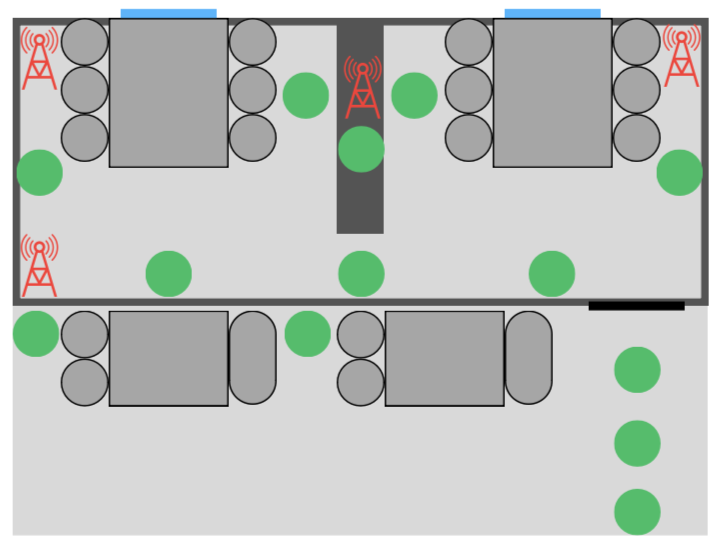
\includegraphics[scale=0.5]{images/experiment_setup.png}
    \caption{A sketch of the meeting room in which the experiments were carried out, decorated with beacon placements (red antenna) and measurement locations (circles with letters)}
    \label{fig:experiment_setup}
\end{figure}

As described in Section \ref{sec:bluetooth_low_energy}, physical obstacles can cause fluctuations in the received signals. 
Therefore, we designed the expirement such that classifcation measurements are taken in areas where some, none, or all of the beacons are blocked by physical obstacles. 
We performed evaluations of the measurements in the following \textit{classification points}:
\begin{itemize}
    \item Along the walls inside of the meeting room, to examine border values of the map while inside the room (see Figure \ref{fig:experiment_setup}, measurement locations A, B, D, F, and G).
    \item Along both sides of the divider, to examine whether obstructions inside the room has any meaningful effect on the classification (E and C).
    \item $1$ meter, $2$ meters, and $3$ meters outside the door, to examine how far away from the meeting a receiver must be before it is classified as outside (see Figure \ref{fig:experiment_setup}, measurement locations J, K, and L).
    \item By the tables in the common area, to ensure that we do not classify an outside area as an inside area (see Figure \ref{fig:experiment_setup}, measurement locations H and I).
\end{itemize}
For each of these areas, 10 data points have been collected and classified on several devices: Samsung Galaxy S20, Samsung Galaxy A53 (also used to create the map), Lenovo TabM10 FHD Plus.
Data collection points and beacon placements in the room during the experiment are illustrated in Figure \ref{fig:experiment_setup}. 

During this second phase, the experimenter used the developed functionality, and the map created in phase one, at each of the classification points to classify incoming signals.
During the classification experiment, k-values of $2,3$ and $4$ and a threshold of $0.5$ were selected to evaluate various configurations of the kNN-based classification algorithm.
This threshold means that more than half of the neighbors of the received measurement need to be classifed as \textit{inside} for it to be classified as \textit{inside}.

While the room was unused during the creation of the map, this was not the case for this part of the experiment.
Computers and phones were placed near the tables of the room, with several of them having either only WiFi, or both Bluetooth and WiFi, enabled. 
In the common area outside the room, two people were tasked with moving around, and a laptop with Bluetooth and WiFi enabled was placed on one of the tables.
This was done to create an environment that more accurately represents a meeting room in use.
The classification context must be considered when establishing whether fingerprinting is a viable approach for the stakeholder - if an unrealistic experimental configuration is used, the results might not translate for the configuration of the stakeholder's meeting rooms. 
Similarly, multiple devices must be used to understand whether the approach is viable only for the device used to create the map, or if a solution requires the stakeholder to provide employees with specific devices. 
During this experiment, three different devices were selected for experimentation: a Samsung Galaxy A53~\cite{a53phone}, Samsung Galaxy S20~\cite{galaxy20phone} phones, and a Lenovo Tab M10 FHD Plus~\cite{tablet} tablet. 
The devices and their Bluetooth specifications are shown in Table \ref{tab:devicesAndBluetooth}.

\begin{table}[h!]
    \resizebox{\textwidth}{!}{%
    \begin{tabular}{|l|l|l|l|l}
    \cline{1-4}
    Device name                & Samsung Galaxy A53 & Samsung Galaxy S20 & Lenovo Tab M10 FHD Plus &  \\ \cline{1-4}
    \textbf{Bluetooth version} & 5.1                & 5.0                & 5.0                     &  \\ \cline{1-4}
    \end{tabular}%
    }
    \caption{The devices used in during classification and their supported Bluetooth version.}
    \label{tab:devicesAndBluetooth}
\end{table}

During the experiment, the experimenter stands in one of the location shown on Figure \ref{fig:experiment_setup}, and uses the developed application to perform $10$ classifications using the previously described threshold.
This process is repeated for each devices, giving a total of $210$ measurements for each k-value.